\chapter{Introducción}
\label{chap:introduccion}

\lettrine{A}{partir} de la segunda década de los 2000, las redes sociales han experimentado
un crecimiento continuado de su uso, tanto en número de usuarios como en
cantidad de información generada. Como se muestra en el reporte \textit{"Digital 2023 Global Overview Report"} (We Are Social et al., 2023)
\cite{wearesocial}, a principios del año 2013 existían alrededor de 1.7 millones de usuarios en las redes sociales,
mientras que a principios del año 2023, esta cifra aumentó hasta los 4.7 millones, con una variación anual media del 10.8\% (se puede ver
más información en la Figura \ref{fig:usuarios_redes_sociales}).
Así, plataformas como Facebook, Instagram, Twitter o YouTube, cuentan con millones de usuarios activos diariamente,
donde se comparte información o se crea contenido de entretenimiento. Además, las redes sociales se han convertido en
un lugar donde se debate sobre temas políticos, sociales o económicos, y donde se comparten diversas opiniones y noticias. 
Este hecho se puede ver, de nuevo, en el reporte mecionado anteriormente, donde se muestra que el 34.2\% de los usuarios
de redes sociales las utilizan para informarse sobre noticias, el 28.8\% para saber cuales son los temas de actualidad
y el 23.4\% para compartir opiniones y debatir con otros usuarios.

\bigskip
\begin{figure}[H]
	\centering
	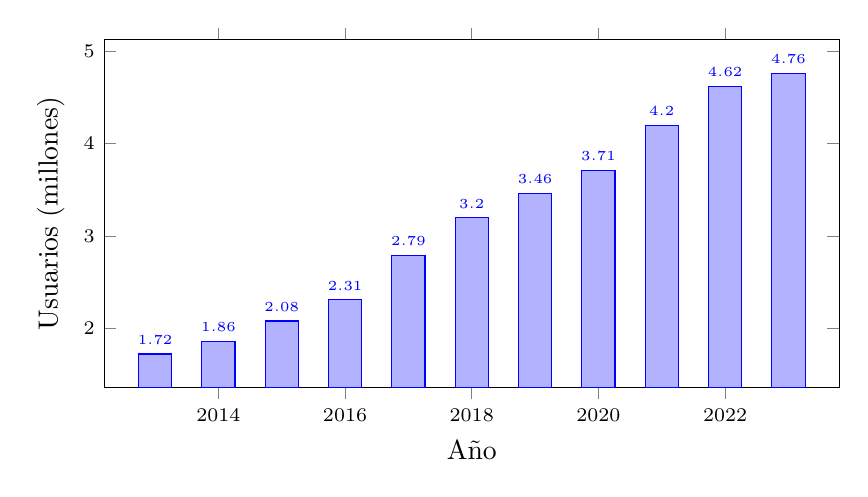
\begin{tikzpicture}
		\begin{axis}[
			width=0.9\textwidth,
			height=6cm,
			xmajorgrids=false,
			x tick label style={/pgf/number format/1000 sep=},
			x tick label style={font=\scriptsize},
			y tick label style={font=\scriptsize},
			ylabel=Usuarios (millones),
			xlabel=Año,
			ybar=6pt,
			bar width=12pt,
			enlarge x limits=0.08,
			enlarge y limits=0.12,
			nodes near coords,
			nodes near coords style={font=\tiny}
		]
		\addplot 
			coordinates {(2013,1.720) (2014,1.857) (2015,2.078)
			(2016,2.307) (2017,2.789) (2018,3.196) (2019,3.461)
			(2020,3.709) (2021,4.199) (2022,4.623) (2023,4.760)};
		\end{axis}
	\end{tikzpicture}
	\caption{Evolución del número de usuarios en redes sociales.}
	\label{fig:usuarios_redes_sociales}
\end{figure}

\section{Importancia de las redes sociales}
\label{sec:intr_importancia}
Toda esta información generada tiene una gran relevancia a distintos niveles. En primer lugar, cabe destacar el impacto que
tienen las redes sociales a nivel político. Y es que en la actualidad, vivimos en una campaña permanente (Blumenthal, 1980)
\cite{sydney1980permanent}, 
donde el acceso a la redes sociales ofrece la posibilidad a los ciudadanos de estar informados sobre política, mientras que a las instituciones
de poder les permite conocer el estado de la opinión pública (Strömbäck, 2008)
\cite{stromback2008four}, pudiendo llegar a influenciar "mucho" o "bastante" la intención de voto (Gallardo-Paúls, 2016)\cite{gallardo2016pseudopolitica}.
En segundo lugar, la información generada en las redes sociales también tiene un gran impacto a nivel social. ¿Quiénes son los
usuarios más activos? ¿Qué género predomina en las redes sociales? ¿Qué edad tienen los usuarios?. Cabe resaltar también el
impacto que tienen las redes sociales a nivel económico, ya que estas plataformas se han convertido en un lugar donde las empresas
publicitan sus productos y servicios y a las que destinan gran parte de sus presupuestos en publicidad 
(Saxena et al., 2013)\cite{saxena2013advertising}. Finalmente, destacar el impacto que tienen las redes sociales a nivel de seguridad,
ya que estas plataformas se han convertido en un lugar donde se comparte información personal, y donde se pueden cometer delitos como
el \textit{cyberbullying} o el \textit{grooming} (Machimbarrena et al., 2018)\cite{machimbarrena2018internet}.

\section{Perfilado de autor}
\label{sec:intro_perfilado}
Surge de esta forma la necesidad de analizar toda la información que se genera y proporiconar así herramientas útiles en todos los niveles vistos en la Sección \ref{sec:intr_importancia}.
En este contexto, el perfilado de autor en redes sociales se ha convertido en un área de investigación de gran interés
en los últimos años, posicionándose como una herramienta de creciente importancia en áreas como la seguridad, el \textit{marketing}
o la investigación forense (Rangel et al., 2013)\cite{rangel2013overview}.

\bigskip
El perfilado de autor, también conocido como \textit{author profiling} en inglés, consiste en determinar, a partir de un texto, 
las características de su autor, como su género, edad, rasgos personales, etc. Para ello se hace uso de diversas técnicas de aprendizaje automático
basadas en NLP (del inglés \textit{Natural Language Processing}), que permiten extraer características lingüísticas del texto y utilizarlas para una
posterior clasificación. Así, el perfilado de autor sería de gran utilidad a la hora de evaluar sospechosos teniendo en cuenta su perfil lingüístico;
sería muy práctico para empresas que quieran conocer el perfil de los clientes que opinan de forma negativa y positiva de sus productos; tendría un gran valor
para los partidos políticos, dado que podrían conocer cuál es el perfil de sus votantes; y sería una herramienta de gran ayuda a la hora de realizar
análisis sociales sobre temas específicos.